\section*{1. Color-magnitude diagram}

\noindent\makebox[\textwidth]{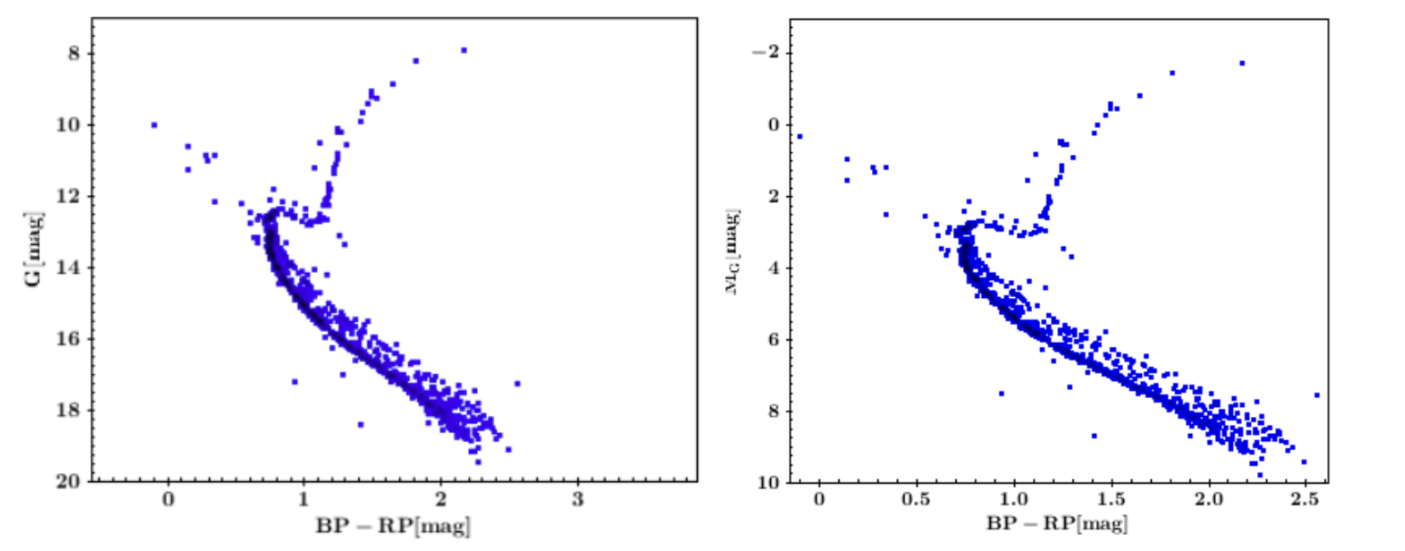
\includegraphics[scale=0.05]{magnitude.png}}\\

Figure 1: Sub-sample of the Gaia data release 3 (DR3) color-magnitude diagram (CMD) in apparent  (left)
and absolute (right) magnitudes. Each dot represents a star and they belong to a stellar cluster. Note:
apparent magnitudes are denoted by $G$, $G_{BP}$ and $G_{RP}$ and absolute magnitudes denoted by $M_G$, 
$M_{G_{BP}}$ and $M_{G_{RP}}$.\\
\\
a) Figure 1 (left) shows the color ($G_{BP} - G_{RP}$) on the x-axis and apparent magnitudes ($G$) on the
y-axis of a group of stars in the Milky Way. The data is taken from a sub-sample of the Gaia data release
3 (DR3). Give a brief description of Photometry. Look up the Gaia mission and give the wavelength 
coverages of the $G$, $G_{BP}$ and $G_{RP}$ passbands.\\
\\
From both diagrams we can identify a clear diagonal, which represents the main sequence. The 
stars in said main sequence are the ones which are in the phase of burning hydrogen. With the x-axis 
values we can determine or at least make assumptions about the color of the stars. With $BP - RP$ we can 
assume that stars to the left are more blueish and stars to the right of the x-axis are more reddish.
Generally speaking stars that emmit blue light tend to be hotter than ones that emmit red light. With that
in mind and taking a look at the y-axis we can further support that because we see that the blue stars 
seem to be brighter than the red ones. The wavelength coverage of $G$ is about 330 to 1050 nanometers, the 
coverage of $G_{BP}$ is the blue spectrum, which is around 450 to 495 and of $G_{RP}$ it is the red 
spectrum, which is 620 to 750 nanometers.\\
\\
b) A color-magnitude diagram (CMD) is a way to sort stars by brightness and temperature. What axis of the
plot is a proxy for brightness? What direction of this axis represents increasing brightness? What axis
of the plot is a proxy for temperature? What direction of this axis represents increasing temperature?\\
\\
The y-axis of the plot is a proxy for brightness. This axis represents the magnitude of stars, which is 
a measure of their brightness. Moving upwards along the y-axis represents increasing brightness. Stars 
located higher on the CMD are generally brighter. The x-axis of the plot is a proxy for temperature. This 
axis represents a color index or spectral type, both of which provide information about the temperature 
of stars. Moving to the left along the x-axis represents increasing temperature. Bluer stars (with lower 
color indices or hotter spectral types) are found on the left side of the CMD, indicating higher 
temperatures.\\
\\
c) On the left plot, label and describe the following components (stellar evolutionary stages): 1) main
sequence, 2) main sequence turn-off, 3) horizontal branch, 4) blue stragglers, and 5) red giants.\\
\\
As previous stated we can see the 1) main sequence as the dark plotted diagonal in about the middle of 
the plot. The 2) main sequence turn-off is the point on the main sequence where stars begin to evolve away 
from the main sequence. That would around the area where the data points or stars begin to have a lower 
magnitude than 12.5 as these data points start to malform the diagonal. The 3) horizontal branch is a 
region populated by stars that have evolved off the main sequence, typically after exhausting their core 
hydrogen. Most of the stars with about a lower magnitude than 12.5 would be in that region as they are 
clearly not part of the main sequence. 4) Blue stragglers are stars that appear to be younger or more 
massive than their surroundings. Those are outliers deviating from the expected evolutionary track or the
right branch of the stars with a lower magnitude than 12.5. 5) Red giants are evolved stars that have 
exhausted the hydrogen in their cores and expanded. They appear on the CMD as bright and reddish. Again
stars on the top right branch that evolves to the right would be counted as red giants.\\
\\
d) The right plot shows the same CMD as the left, but the apparent magnitudes have been converted to
absolute magnitudes. Using the plot write down the apparent and absolute magnitudes of the main sequence
turn-off points. Use the distance modulus formula to find the approximate distance to this stellar 
cluster.\\
\\
The apparent magnitude of the MSTO as $m_{MSTO}$ is as previous stated about 12.5 and the absolute 
magnitude as $M_{MSTO}$ is around 2.5. The distance modulus formula is:
\begin{equation*}
  \begin{split}
    m - M &= 5 log_{10}(\frac{d}{10})\\
    \frac{1}{5} (m - M) &= log_{10}(\frac{d}{10})\\
    10^{\frac{1}{5} (m - M)} &= \frac{d}{10}\\
    d &= 10^{(\frac{1}{5} (m - M) + 1)}
  \end{split}
\end{equation*}
Inserting the values no we get:
\begin{equation*}
  \begin{split}
    d &= 10^{(\frac{1}{5} (m - M) + 1)}\\
      &= 10^{(\frac{1}{5} (12.5 - 2.5) + 1)}\\
      &= 10^{(\frac{1}{5} (10) + 1)}\\
      &= 10^{(2 + 1)}\\
      &= 10^{3}\\
      &= 1000\\
  \end{split}
\end{equation*}
The distance is about 1000 parsec.
